%implementing document formatting:
\documentclass[12pt,twoside,a4paper]{report}

% Select encoding of your inputs
\usepackage[utf8]{inputenc}

% Make latex understand and use the typographic
% rules of the language used in the document.
\usepackage[english]{babel}

% Use the vector font Latin Modern which is going
% to be the default font in latex in the future.
\usepackage{lmodern}

% Choose the font encoding
\usepackage[T1]{fontenc}

% Use color in tables
\usepackage[table]{xcolor}
\usepackage{array}
\usepackage{multirow}

% Load a colour package
\usepackage{xcolor}
\definecolor{aaublue}{RGB}{33,26,82}  %<--define aaublue
\definecolor{white}{RGB}{255,255,255} %<--define white

% The standard graphics inclusion package
\usepackage{graphicx}

\makeatletter
  \g@addto@macro\@floatboxreset\centering %<--centering all figures
\makeatother

\usepackage{adjustbox}

% Set up how figure and table captions are displayed
\usepackage{float}
\usepackage{caption}
\usepackage{subcaption}
\captionsetup
{
  justification = justified,         %<--centering caption with multiple lines
  font          = footnotesize, %<--set font size to footnotesize
  labelfont     = bf            %<--bold label (e.g., Figure 3.2) font
}
\captionsetup[subfigure]
{
  justification = centering, %<--centering subfigure caption text
  singlelinecheck=false,
  font = footnotesize        %<--font size for subfigures
} 

% Enable row combination in tables
\usepackage{multirow}

% Make space between table lines and text
\renewcommand{\arraystretch}{1.5}

% Enable commands like \st (strike out) and \hl (high light)
\usepackage{soul}

% Make the standard latex tables look so much better
\usepackage{array,booktabs}

% Enable the use of frames around, e.g., theorems
% The framed package is used in the example environment
\usepackage{framed}
\usepackage{colortbl}
\usepackage{longtable}
\usepackage{xcolor}
\usepackage{textcomp}

%-------MATHEMATICS---------------------------------
% Defines new environments such as equation,
% align and split 
\usepackage{amsmath}
\usepackage{relsize}
% Adds new math symbols
\usepackage{amssymb}
% Use theorems in your document
% The ntheorem package is also used for the example environment
% When using thmmarks, amsmath must be an option as well. Otherwise \eqref doesn't work anymore.
\usepackage[framed,amsmath,thmmarks]{ntheorem}
\usepackage{xifthen}%<--enables ifthenelse which is used in macros

\usepackage{siunitx} 
\sisetup{decimalsymbol=period}%<--\num{} will swich commas with periods
\sisetup{detect-weight}
%---------------------------------------------------

%-------PAGE LAYOUT---------------------------------
% Change margins, papersize, etc of the document
\usepackage[
  left=25mm,% left margin on an odd page %tidligere 25mm for baade right og left
  right=25mm,% right margin on an odd page
  top=35mm,
  ]{geometry}
  
% Modify how \chapter, \section, etc. look
% The titlesec package is very configureable
\usepackage{titlesec}
\makeatletter
\def\ttl@mkchap@i#1#2#3#4#5#6#7{%
    \ttl@assign\@tempskipa#3\relax\beforetitleunit
    \vspace{\@tempskipa}%<<<<<< REMOVE THE * AFTER \vspace
    \global\@afterindenttrue
    \ifcase#5 \global\@afterindentfalse\fi
    \ttl@assign\@tempskipb#4\relax\aftertitleunit
    \ttl@topmode{\@tempskipb}{%
        \ttl@select{#6}{#1}{#2}{#7}}%
    \ttl@finmarks  % Outside the box!
    \@ifundefined{ttlp@#6}{}{\ttlp@write{#6}}}
\makeatother

\titlespacing{\chapter}{0pt}{0pt}{10pt}
\titlespacing{\section}{0pt}{0pt}{-5pt}
\titlespacing{\subsection}{0pt}{8pt}{-5pt}
\titlespacing{\subsubsection}{0pt}{6pt}{-10pt}

\titleformat*{\section}{\normalfont\Large\bfseries\color{aaublue}}
\titleformat*{\subsection}{\normalfont\large\bfseries\color{aaublue}}
\titleformat*{\subsubsection}{\normalfont\normalsize\bfseries\color{aaublue}}

\usepackage{titlesec, blindtext, color}
%\color{gray75}{gray}{0.75}
\newcommand{\hsp}{\hspace{20pt}}
\titleformat{\chapter}[hang]{\Huge\bfseries}{\thechapter\hsp\textcolor{aaublue}{|}\hsp}{0pt}{\Huge\bfseries}

% Change the headers and footers
\usepackage{fancyhdr}
\setlength{\headheight}{15pt}
\pagestyle{fancy}
\fancyhf{} %delete everything
\renewcommand{\headrulewidth}{0pt} %remove the horizontal line in the header
%\fancyhead[RO,LE]{\color{aaublue}\small\nouppercase\leftmark} %even page - chapter title
\fancyhead[LO]{}
\fancyhead[RE]{} 
\fancyhead[CE]{}
\fancyhead[CO]{}
\fancyfoot[RE,LO]{\thepage}
%\fancyfoot[LE,RO]{B205} %page number on all pages
\fancyfoot[CE,CO]{}

% change first page of all chapters header and footer to fancy style
\makeatletter
\let\ps@plain\ps@fancy
\makeatother

% Do not stretch the content of a page. Instead,
% insert white space at the bottom of the page
\raggedbottom

% Enable arithmetics with length. Useful when typesetting the layout.
\usepackage{calc}
%---------------------------------------------------

%-------BIBLIOGRAPHY--------------------------------
%setting references (using numbers) and supporting i.a. Chicargo-style:
\usepackage{etex}
\usepackage{etoolbox}
\usepackage{keyval}
\usepackage{ifthen}
\usepackage{url}
\usepackage{csquotes}
\usepackage[backend=biber, url=true, doi=true, style=numeric, sorting=none]{biblatex}
\addbibresource{setup/bibliography.bib}
%---------------------------------------------------

%-------MISC----------------------------------------
%%% Enables the use FiXme refferences. Syntax: \fxnote{...} %%%
\usepackage[footnote, draft, english, silent, nomargin]{fixme}
%With "final" instead of "draft" an error will ocure for every FiXme under compilation.

%%% allows use of lorem ipsum (generate i.e. pagagraph 1 to 5 with \lipsum[1-5]) %%%
\usepackage{lipsum}

%%% Enables figures with text wrapped tightly around it %%%
\usepackage{wrapfig}

%%% Section debth included in table of contents (1 = down to sections) %%%
\setcounter{tocdepth}{1}

%%% Section debth for numbers (1 = down to sections) %%%
\setcounter{secnumdepth}{1}

\usepackage{tocloft}
\setlength{\cftbeforetoctitleskip}{0 cm}
\renewcommand{\cftpartpresnum}{Part~}
\let\cftoldpartfont\cftpartfont
\renewcommand{\cftpartfont}{\cftoldpartfont\cftpartpresnum}
%---------------------------------------------------

%-------HYPERLINKS----------------------------------
% Enable hyperlinks and insert info into the pdf
% file. Hypperref should be loaded as one of the 
% last packages
\usepackage{nameref}
\usepackage{hyperref}
\hypersetup{%
	%pdfpagelabels=true,%
	plainpages=false,%
	pdfauthor={Author(s)},%
	pdftitle={Title},%
	pdfsubject={Subject},%
	bookmarksnumbered=true,%
	colorlinks,%
	citecolor=aaublue,%
	filecolor=aaublue,%
	linkcolor=aaublue,% you should probably change this to black before printing
	urlcolor=aaublue,%
	pdfstartview=FitH%
}
%---------------------------------------------------

% remove all indentations
\setlength\parindent{0pt}
\parskip 5mm
\usepackage{verbatim}

\definecolor{Gra}{RGB}{230,230,230}

%creates a nice-looking C#-text
\newcommand{\CC}{C\nolinebreak\hspace{-.05em}\raisebox{.3ex}{\scriptsize\text \#} }

%enables multi column lists
\usepackage{multicol}

%enables code-examples
\usepackage{listings}

\definecolor{coolblue}{RGB}{32,95,128}
\definecolor{mygreen}{rgb}{0,0.6,0}
\definecolor{mygray}{rgb}{0.5,0.5,0.5}
\definecolor{mymauve}{rgb}{0.58,0,0.82}
\usepackage{textcomp}
\definecolor{listinggray}{gray}{0.9}
\definecolor{lbcolor}{rgb}{0.9,0.9,0.9}

\lstset{
backgroundcolor=\color{lbcolor},
	tabsize=4,
	rulecolor=,
	language=C,
        basicstyle=\scriptsize,
        upquote=true,
        aboveskip={1.5\baselineskip},
        columns=fixed,
        showstringspaces=false,
        extendedchars=true,
        breaklines=true,
        prebreak = \raisebox{0ex}[0ex][0ex]{\ensuremath{\hookleftarrow}},
        frame=single,
        showtabs=false,
        numbers=left,
        captionpos=b,
        numbersep=5pt,
        numberstyle=\tiny\color{mygray},
        showspaces=false,
        showstringspaces=false,
        identifierstyle=\ttfamily,
        keywordstyle=\color[rgb]{0,0,1},
        commentstyle=\color[rgb]{0.133,0.545,0.133},
        stringstyle=\color[rgb]{0.627,0.126,0.941},
}

\usepackage{enumitem}
%\usepackage[citestyle=authoryear,natbib=true]{biblatex}

% Figures - TIKZ
\usepackage{tikz}
\usepackage[americanresistors,americaninductors,americancurrents, americanvoltages]{circuitikz}

% Wall of text logo
\newcommand{\walloftextalert}[0]{\includegraphics[width=\textwidth]{walloftext.png}}

\usepackage{pdfpages}
\usepackage{lastpage}
\usepackage{epstopdf}

\setlength{\headheight}{21pt}

\hfuzz=\maxdimen
\tolerance = 10000
\hbadness  = 10000

\usepackage{siunitx}
\graphicspath{{./figures/}}
%Vectors
\renewcommand{\vec}[1]{\boldsymbol{\mathbf{#1}}}
\begin{document}
\renewcommand\chaptername{KAPITEL}
\renewcommand\contentsname{Indhold}
\renewcommand\figurename{Figur}
\renewcommand\tablename{Tabel}

\section*{Review of Paper on\\
Networked Control for Water Distribution\\
\small Wednesday, 30th of November 2016}
\subsection{Overall Assessment}
Very nice paper to read. Understandable and good flow of information. \\
There are some spelling and grammatical errors, which needs to be looked into.  
\subsection{General Comments}
\begin{itemize}
	\item[-] Maybe the abstract should also contain the conclusion of the project, to give a full first impression of the project.
	\item[-]There are different ways of implementing equations in the flow of the paper. However, we think that including the equations as part of the sentences provides a good flow. In this case, proper grammatical punctuation should be used around equations.\\
\begin{figure}[H]
    \centering
    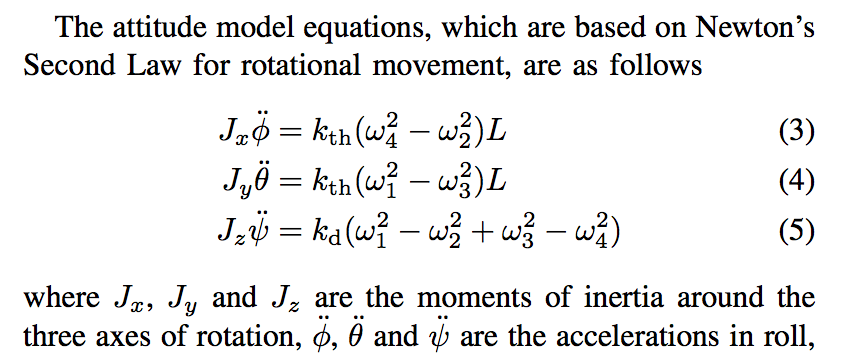
\includegraphics[width=.4\textwidth]{equation.PNG}
\end{figure}
Either way, we suggest to select one way and then stick to it as much as possible. Right now you change between using a colon and not using a colon. 
\item[-]Using "below" and "above" for figure and equation references can be confusing in a paper where the layout is in columns, we think that the figure reference itself is sufficient.
\end{itemize}	
\subsection{Specific Comments}
\begin{itemize}
\item[-]The headline, we suggest, should be written as: Networked Control for Water Distribution.
\item[-]Abstract - 1st column - 1st paragraph - "Water Distribution networks are play a key infrastructure role for cities and industrial areas around the world."\\
Suggestion: "Around the world water distribution networks have a key role for cities and industrial areas infrastructure."\\
\item[-]Abstract - 1st column - 1st paragraph - "The nature of water distribution networks means the actuators, sensors and control systems are geographically separated [...]".\\
Suggestion: "in general water distribution networks have actuators, sensors and control systems geographically separated [...]".\\
\item[-]Section I - 1st column - 2nd paragraph - "[...] distribution networks (WDN) so all consumers [...]".\\
Suggestion: "[...] distribution networks (WDN) to ensure all consumers [...]".\\
\item[-] Section I - 1st column - 2nd paragraph - "Addition of users in a network [...]".\\
Thoughts: We don't know if you mean "Adding  users to the network [...]" or "In addition to the users in the network [...]" \\
\item[-]Section I - 1st column - 2nd paragraph - "[..] in whole distribution network [..]".\\
Suggestion: "[...] in the whole distribution network. [...]".\\
\item[-]Section I - 1st column - 2nd paragraph - "[...] according to consumer's need and components available in that network [...]".\\
Suggestion: "[...] according to  consumer's needs and the components available in the specific network [...]".\\
\item[-]Section I - 1st column - 2nd paragraph - "[...] desired operating pressure point via [...]".\\
Suggestion: "[...]desired pressure operating point by utilizing [...]".\\
\item[-]Section I - 1st column - 2nd paragraph - "The water distribution network has nonlinear characteristics [3]".\\
Suggestion: This sentence is slightly out of context, maybe including it in the Section II description underneath (3rd paragraph in section I), as a reason to linearize, would be better.\\
\item[-]Section I - 1st column - 3rd paragraph: " [...] and state space model is derived from linearized model [...]".\\
Suggestion: "[...] and "a" state space model is derived from "a" linearized model [...]".\\
\item[-]Section I - 1st and 2nd column - 3rd paragraph: "In section III [...]".\\
Suggestion: This should be on the same line and column.\\
\item[-]Section II A 1 - 2nd column - paragraph 2: "Includes the surface resistance and from resistance".\\
Thoughts: What is this "from resistance"?\\
\item[-]Thoughts on Section II A 1 - 2nd column - equation (1)\\
Note: It is hard to see that it is an absolute value of $q_k$. \\

\item[-]Section II C - 2nd column - 2nd paragraph - Figure 1\\
Suggestion: Nice figure, maybe the three components can be in a row to take up less space.\\
\item[-]Section II C - 2nd column - 4th paragraph - "[...] component in the network and the components are in reference to Figure 1."\\
Suggestion: "[...] component in the network."\\
\item[-]Section II C - 1st and 2nd column - 4th paragraph - Figure 4\\
Thoughts: The figure is really nice. However it is quite small; maybe it could take up an entire page, if there is enough room for it.\\
\item[-]Section II C - 1st and 2nd column - 4th paragraph - Figure 4 - Figure text: "Test Water Distribution Network Diagram".\\
Suggestion: "Diagram of the water distribution network test setup."\\
\item[-]Section II C - 1st column - 6th paragraph - "[...] for the pipe, valve from [...]".\\
Suggestion: "[...] for the pipe and valve from [...]".\\
\item[-]Section II C - 1st column - 6th paragraph - "[...] are shown below. [enter] Thus, in matrix form, [...]".\\
Thoughts: You write like there are loop equations below (which there aren't).\\
\item[-]Section III - 1st column - 3th paragraph - Figure 5: The label and title should be bigger. Furthermore a legend should be included.\\
\item[-]Section - 1st column - 4th paragraph - "Figure 5. above, the system's output [...]"\\
Suggestion: "In Fig. 5, the system's output [...]"\\
Thought: As it is referred to Fig. 5 in the figure, therefore it should be Fig. 5 in the text as well.\\
\item[-]Section IV - 1st column - 1st paragraph: "This introduced the delays from sensors to controlling part and also from controlling parts to actuators."\\
Suggestion: "This introduces delays from sensors to controllers and from controllers to actuators."\\
\item[-]Section IV - 1st column - 1st paragraph: "[...] delay is occurred in system by controllers, actuators and network controlling part exchanging data."\\
Suggestion: "[...] delay occurs when the different components of the system, the controller, actuators and sensors, are exchanging data."\\
Thoughts: Maybe we do not understand it correctly, in which case it should be written more clearly.\\
\item[-]Section IV - 1st column - 1st paragraph: "[...] compared to other."\\
Thoughts: Other?
\end{itemize}
\end{document}